\documentclass[]{article}
\usepackage{polski}
\usepackage[utf8]{inputenc}
\usepackage{amsmath}
\usepackage{graphicx}
\usepackage{geometry}
\usepackage{float}

\geometry{legalpaper, margin=0.6in}

%opening
\title{AMO - Projekt 1, zestaw 25}
\author{Jakub Postępski}

\begin{document}

\maketitle


\section{Układ równań współrzędnych kartezjańskich}
Dla każdego punktu w układzie współrzędnych "geograficznych" mamy:
\[ x = r\cos \theta \cos \phi \]
\[ y = r\cos \theta \sin \phi \]
\[ z = r\sin \theta \]
gdzie $ \theta $ to długość geograficzna i $ \phi $ to szerokość geograficzna.

Dla każdego punktu w układzie współrzędnych kartezjańskich mamy:
\[ r = \sqrt{x^2 + y^2 + z^2}\]
\[ \theta = \arctan \frac{y}{x} \]
\[ \phi = \arcsin \frac{z}{r} \]


\section{Zadanie optymalizacji}
Należy zminiamalizować sumę kwadratów funkcji $f(x)$ wyrażających błąd pomiędzy zmierzonym a rzeczywistym czasem dotarcia sygnału z satelit do odbiornika.

\[ \min || f(x) ||^2_2 = \min (f(x_1)^2 + ... + f(x_5)^2)\]

dla funkcji:

\[ f(x_i) = \sqrt{(x-x_i)^2 + (y-y_i)^2 + (z-z_i)^2}-t_iC\]

gdzie:
\begin{itemize}
	\item $x$, $y$, $z$ to wsp. szukanego punktu
	\item $x_i$, $y_i$, $z_i$ to wsp. odpowiedniego satelity
	\item $t_i$ to zmierzony czas dotarcia sygnału z satelity
	\item $C$ to stała określająca prędkość światła
\end{itemize}

\section{Jakobian}
Ponieważ współrzędne satelitów zdefiniowane są w układzie "geograficznym" a zadanie optymalizacji jest zdefiniowane w układzie współrzędnych kartezjańskich zastosowano jakobian z wierszami postaci:
\[J_i = \begin{bmatrix}
	\frac{x - x_i}{\sqrt{(x_i - x)^2 + (y_i - y)^2 + (z_i - z)^2}} &
	\frac{y - y_i}{\sqrt{(x_i - x)^2 + (y_i - y)^2 + (z_i - z)^2}} &
	\frac{z - z_i}{\sqrt{(x_i - x)^2 + (y_i - y)^2 + (z_i - z)^2}}
\end{bmatrix} \]

\section{Rozwiązanie zadania}
Oba programy (Matlab oraz AMPL) wyznaczyły to samo położenie
\[ \theta = 51.3759 , \phi = 21.3779 \] i tą samą wysokość nad poziomem morza ($172$ m).

\section{Google Maps}
\begin{figure}[H]
	\centering
	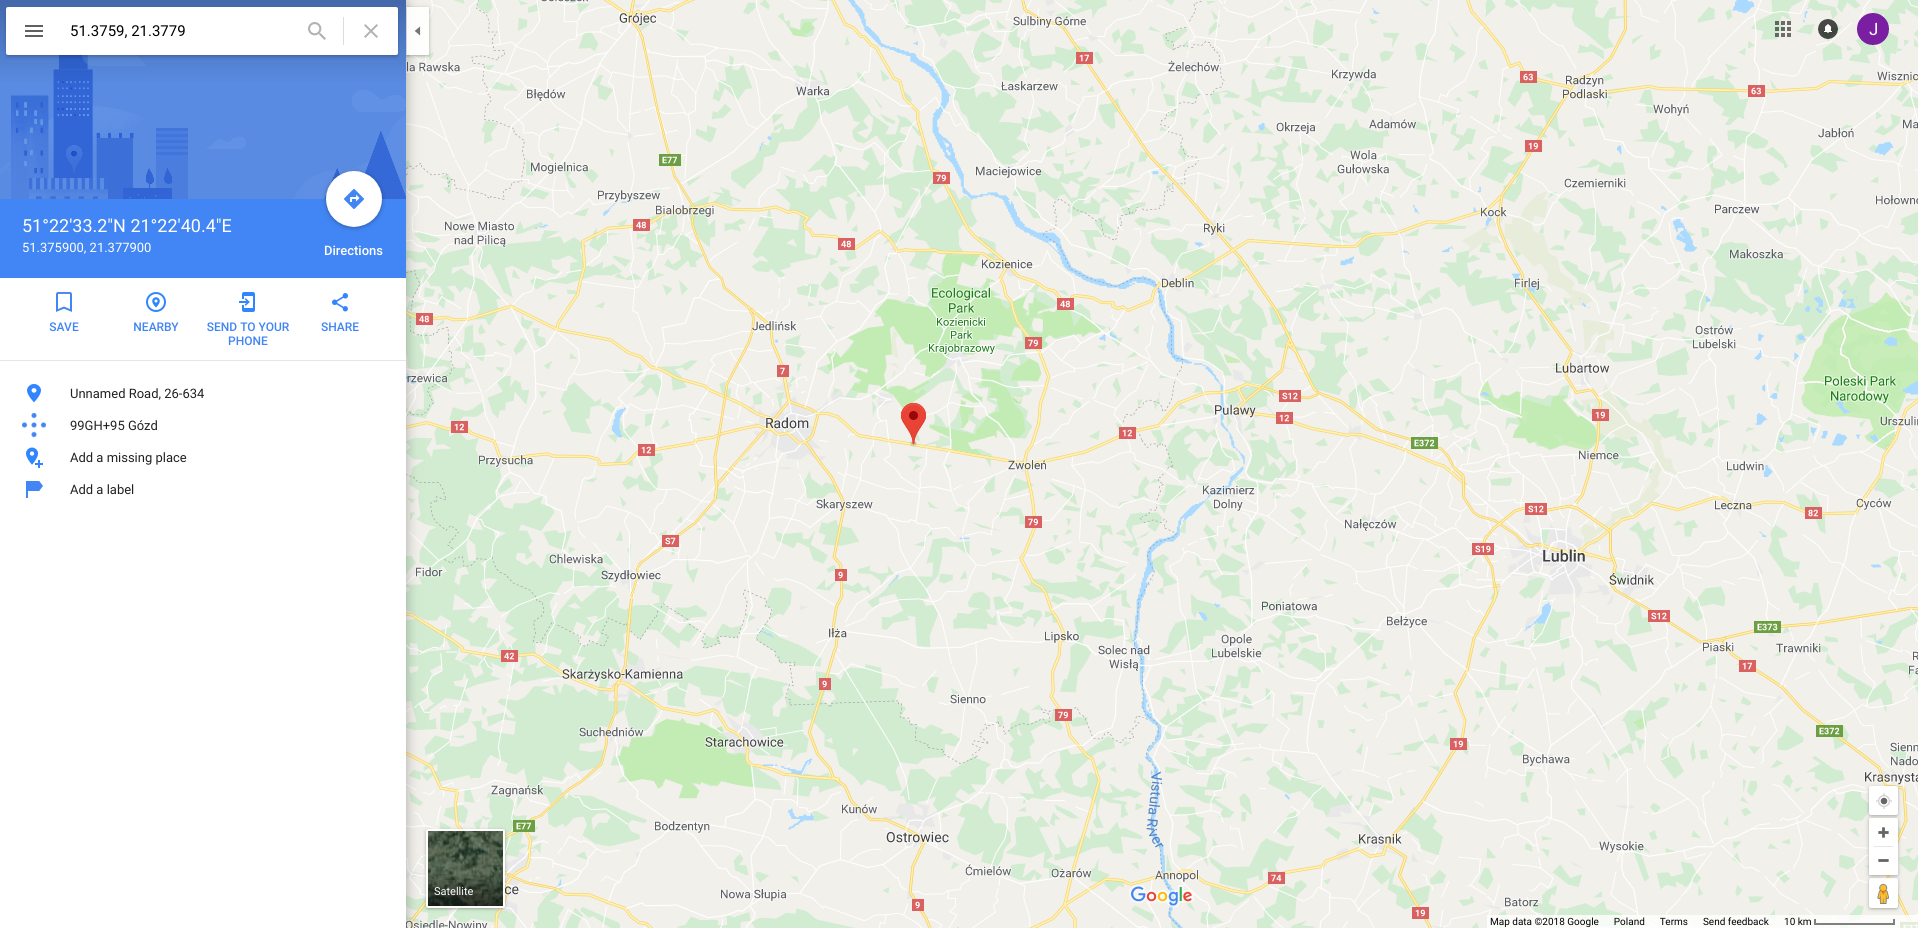
\includegraphics[width=0.99\linewidth]{daleko}
	\caption{Widok daleki znalezionego punktu}
	\label{fig:daleko}
\end{figure}

\begin{figure}[H]
	\centering
	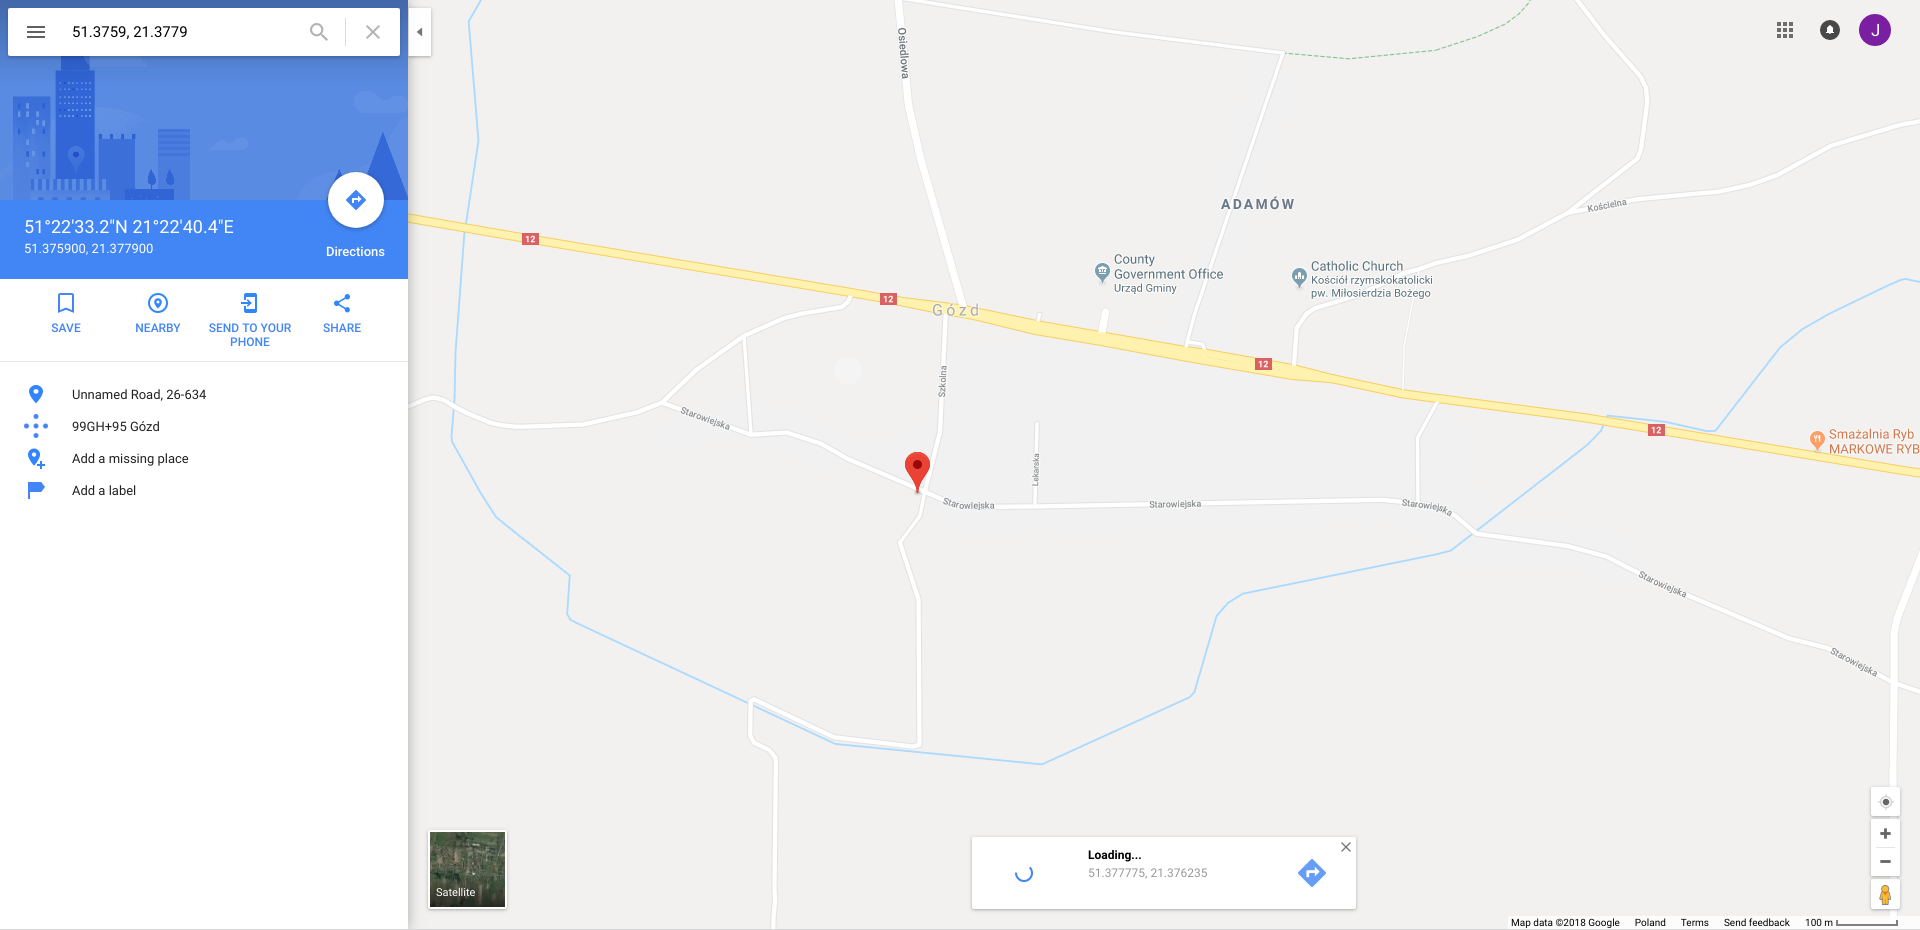
\includegraphics[width=0.99\linewidth]{blisko}
	\caption{Widok miejscowości znalezionego punktu}
	\label{fig:blisko}
\end{figure}

\section{Zmiana parametrów optymalizacji}
Na początku zastosowano domyślny algorytm Trust Region Reflective, który zatrzymywał się po 22 iteracjach.

Algorytm Levenberga-Marquardta (stosowany do dalszych badań) zatrzymał się po 4 iteracjach, co świadczy o jego znacznej przewadze. Po podaniu jakobianu
algorytm zatrzymał się także po 4 iteracjach. Algorytm generuje większy błąd względny.

Wyniki błędów algorytmu dla różnych parametrów przedstawia tabela \ref{tab1}. Co oczywiste przy zaburzaniu danych wejściowych algorytmów wynik optymalizacji też się zmieniał.

\subsection{Zmiana punktu startowego}
Po zadaniu punktu startowego, którego współrzędne były bardzo dużymi liczbami liczba iteracji algorytmu zwiększyła się do 5. Uzyskany wynik zawsze był taki sam.
\subsection{Zmiana warunku stopu}
Domyślna tolerancja pozwala na uzyskanie dość dokładnych wyników. Wykonywane jest wtedy 4 iteracji algorytmu. Od 3 iteracji możemy uznać, że uzyskane wyniki są dość dokładne.

Zmniejszanie domyślnej tolerancji algorytmu nie spowodowało wykonania dodatkowych iteracji algorytmu. Oznacza to, że błędy numeryczne nie pozwalają uzyskać większej dokładności niż domyślna.

Zwiększanie tolerancji do $10^{-5}$ nie spowodowało znaczącej zmiany wyniku optymalizacji. Dalsze zmniejszanie tolerancji spowodowało zmniejszenie dokładności przez fakt wykonania mniejszej liczby iteracji algorytmu. Ustawienie tolerancji większej od $1$ powoduje, że wykonanie algorytmu nie ma sensu.

\subsection{Zaburzanie danych wejściowych}
Do eksperymentów zaburzano parametry piątego satelity. Zmiana szerokości i długości geograficznej do 10 \% nie powoduje dużej zmiany wyniku. Większe zmiany powodują znaczne zmiany. Algorytm jest dużo bardziej czuły na zmiany czasu przesyłu. Zmiana o 5 \% powoduje znaczny błąd optymalizacji. Wynika to z definicji problemu optymalizacji. Promień sfery definiowany czasem ma duży wpływ na całe obliczenia.

\begin{table}[H]
	\begin{tabular}{||c c c c c | c c||}
		\hline
		L. p. & Zmiana $\theta$ & Zmiana $\phi$ & Zmiana $t$ & Inne zmiany & Liczba iteracji & Błąd względny \\ [0.5ex]
		\hline\hline
		1 & b. z. & b. z. & b. z. & Algorytm True Reflective Region & 22 & 4.1633e-17 \\
		\hline
		2 & $\times-1.2$ & b. z. & b. z. & Algorytm True Reflective Region & 22 & 6.9544e+10 \\
		\hline
		3 & b. z. & b. z. & b. z. & b. z. & 4 & 4.0503e-09 \\
		\hline
		4 & $\times-1.2$ & b. z. & b. z. & b. z. & 4 & 2.1051e+13 \\
		\hline
		5 & $\times-1.5$ & b. z. & b. z. & b. z. & 4 & 5.8005e+13 \\
		\hline
		6 & $\times1.2$ & b. z. & b. z. & b. z. & 4 & 2.9344e+09 \\
		\hline
		7 & $\times1.5$ & b. z. & b. z. & b. z. & 4 & 1.9436e+10 \\
		\hline
		8 & b. z. & $\times-1.2$ & b. z. & b. z. & 4 & 3.8917e+08 \\
		\hline
		9 & b. z. & $\times1.5$ & b. z. & b. z. & 4 & 2.9201e+09 \\
		\hline
		10 & b. z. & b. z. & $\times1.05$ & b. z. & 4 & 1.9876e+11 \\
		\hline
		11 & b. z. & b. z. & $\times1.2$ & b. z. & 4 & 3.3333e+12 \\
		\hline
		12 & $\times1.2$ & $\times1.2$ & $\times1.2$ & b. z. & 4 & 5.9120e+11 \\
		\hline
		13 & b. z. & b. z. & b. z. & Zmiana punktu startowego & 5 & 4.0503e-09 \\
		\hline
		14 & b. z. & b. z. & b. z. & Zwiększenie tolerancji & 3 & 2.0317e+09 \\
		\hline
	\end{tabular}
	\caption{Eksperymenty zaburzające parametry wejściowe funkcji lsqnonlin() dla piątego satelity.}
	\label{tab1}
	\end{table}

\end{document}
